\documentclass[a4paper]{article} % For LaTeX2e
\usepackage[T1]{fontenc} % add special characters (e.g., umlaute)
\usepackage[utf8]{inputenc} % set utf-8 as default input encoding
\usepackage{ISMIRlbd, cite, times, amsmath, url}
\usepackage{hyperref}
\usepackage{url}
\usepackage{float}
\usepackage{graphicx}
\usepackage{booktabs}
\usepackage{color}
\usepackage{amsfonts}

\title{\MakeLowercase{flow}EQ: A smarter equalizer plugin using the $\beta$-VAE}


% Note: Please do NOT use \thanks or a \footnote in any of the author markup

% Single address
% To use with only one author or several with the same address
% ---------------
%\oneauthor
% {Names should be omitted for double-blind reviewing}
% {Affiliations should be omitted for double-blind reviewing}

% Two addresses
% --------------
%\twoauthors
%  {First autho} {School \\ Department}
%  {Second author} {Company \\ Address}

%% To make customize author list in Creative Common license, uncomment and customize the next line
\def\authorname{Christian Steinmetz, Xavier Serra}

\oneauthor
  {Christian Steinmetz  Xavier Serra} {Music Technology Group, Universitat Pompeu Fabra, Barcelona (Spain) \\ {\tt christian.steinmetz@upf.edu}}

\newcommand{\fix}{\marginpar{FIX}}
\newcommand{\new}{\marginpar{NEW}}

%\iclrfinalcopy % Uncomment for camera-ready version, but NOT for submission.
\begin{document}


\maketitle

\begin{abstract}

% [ main abstract ]

We present flowEQ, an intelligent interface for a five-band parametric equalizer plugin. 
This tool enables the audio engineer to control all thirteen parameters of the equalizer using either one, two, or three sliders. 
This is achieved by learning low dimensional mappings from one, two, and three dimensional latent spaces to the thirteen dimensional parameter space of the equalizer. 
We use a disentangled variational autoencoder ($\beta$-VAE) trained on a dataset of equalizer configurations collected from audio engineers. 
Different levels of latent space disentanglement are investigated, providing the user with the ability to adjust the latent representations directly within the plugin. 
By traversing the latent spaces of the trained models, the user can quickly search through relevant configurations of the equalizer. 
This enables both novice and experienced audio engineers to more efficiently apply timbral processing during post-production.

% [ plugin screenshot ]

\begin{figure}[H]
  \centerline{
  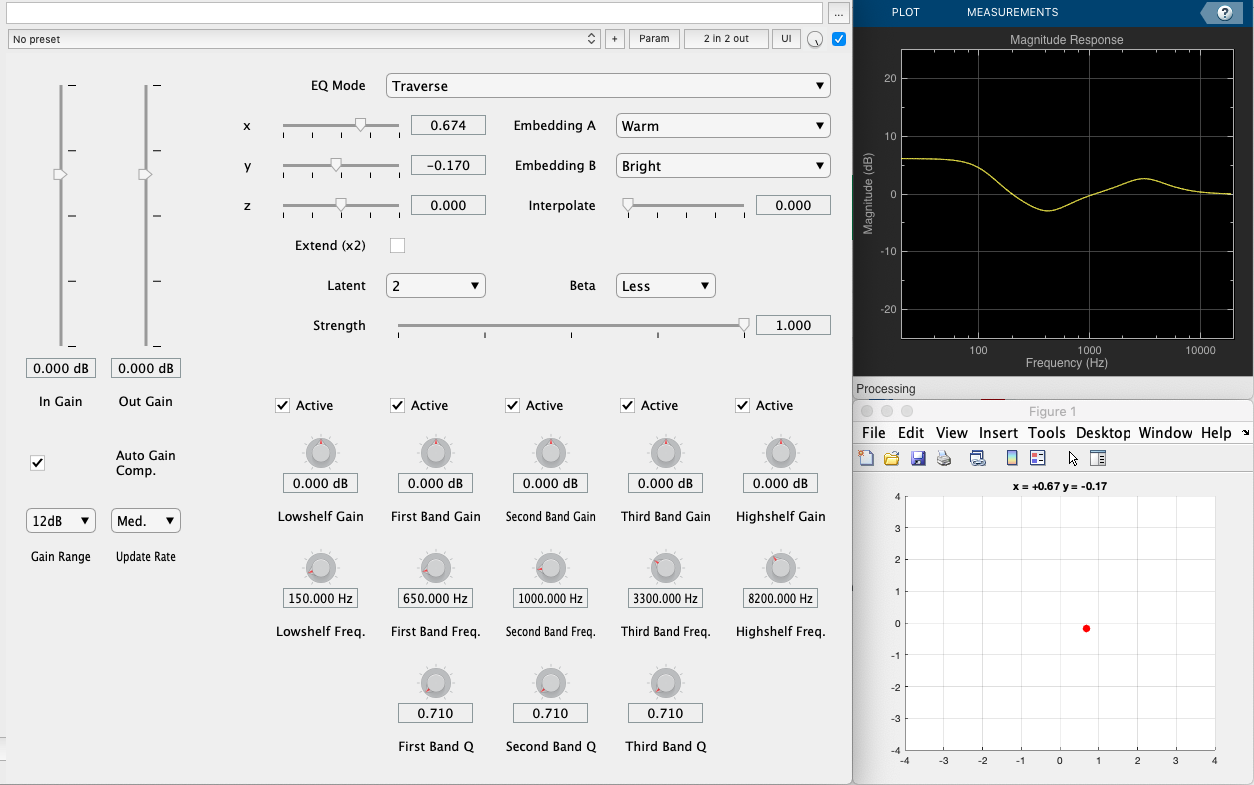
\includegraphics[width=0.5\columnwidth]{../../img/full_visual.png}}
  \caption{VST plugin running in REAPER with real-time MATLAB visualization tool.}
  \label{fig:plugin}
 \end{figure}

% [ introduction ]

The parametric equalizer is the de-facto tool used by audio engineers to shape the timbre of an audio signal. 
First employed with analog circuitry in the early 1970s \cite{massenburg}, these processors have evolved with the advent of digital signal processing, and are readily available as plugins or standalone outboard processors. 
Providing direct control over the gain, center frequency, and bandwidth (known as Q factor) for each band, the parametric equalizer is one of the most powerful forms of the equalizer. 
Due to this increased complexity, experience is required on the part of the audio engineer in order to achieve the desired timbral effect. 
Our goal is to provide a simplified interface to efficiently search across relevant configurations of the equalizer without extensive experience. 

% [ previous work ]

Previous work has investigated the use of timbral semantics for the intelligent control of equalizers. 
In \cite{cartwright_socialeq}, the authors collect and analyze crowdsourced data to uncover universal, semantic descriptors of timbre, with the goal of designing an equalizer that can respond to descriptive language. 
The SAFE project \cite{safe2014} introduces compression, distortion, reverb, and parametric equalization plugins, which provide a means to collect semantic data directly from the normal workflow of audio engineers. 
The work presented in \cite{stasis_reduce_dimension} is the most similar to ours. 
They use data from the SAFE project and employ a number of classical dimensionality reduction techniques to build a model that attempts to control the ‘warmth’ and ‘brightness’ of an equalizer. 

While these semantic interfaces present potentially promising results in the control of an equalizer, they are inherently limited by the generalization and relative specificity of the semantic descriptors studied. 
flowEQ expands upon this work by employing a more modern and powerful model, the variational autoencoder, along with the investigation of variable latent space dimensionality and disentanglement. 

% [ method ]

We use the VAE formulation originally presented in \cite{vae}, where we attempt to jointly learn the parameters, $\phi$ and $\theta$, of a probabilistic encoder, $q_\phi(\mathbf{x}|\mathbf{z})$, and a generative decoder, $p_\theta(\mathbf{z}|\mathbf{x})$.
During optimization we minimize the expected negative log-likelihood for the data generated by the decoder, after sampling a latent code from the encoder. 
This acts as a reconstruction loss, incentivising the model to accurately encode and decode the equalizer parameters. 
We assume the latent prior is gaussian, such that $p(\mathbf{z}) = \mathcal{N}(0,1)$. 
We then utilize the KL divergence between the encoder, $q_\phi(\mathbf{x}|\mathbf{z})$, and the prior, as a regularizer, which incentivizes the encoder to learn well structured latent mappings. 

\begin{equation}
  \mathcal{L}(\pmb{\theta},\pmb{\phi},\mathbf{x}^{(i)}) = - \mathbb{E}_{\mathbf{z} \sim q_{\theta}(\mathbf{z}|\mathbf{x}^{(i)})} [ {\log{p_\phi(\mathbf{x}^{(i)} | \mathbf{z})}} ] + \mathbf{\beta} \: D_{KL} (q_\theta(\mathbf{z} | \mathbf{x}^{(i)}) || p(\mathbf{z})).
  \label{eq:loss}
\end{equation}

Equation \ref{eq:loss} shows the loss function, with the addition of a hyperparameter, $\beta$, known as the disentanglement factor \cite{higgins_betavae}. 
Adjusting $\beta$, the relative weight of the reconstruction and KL loss, allows us to investigate different levels of latent space disentanglement.
Greater disentanglement means the latent space is structured so that each dimension more closely models a single characteristic of the data. 
We train a total of twelve different models with three different latent space bottlenecks (1D, 2D, and 3D), each with one of four values of $\beta$.

% [ implementation ] 

The plugin is implemented with the MATLAB Audio Toolbox\footnote{\url{https://www.mathworks.com/products/audio.html}}, which provides an API for compiling MATLAB code directly to VST/AU plugins. 
Compiled plugins for macOS and Windows are made available on the project website\footnote{\url{https://flowEQ.ml/}}, as well as the source code\footnote{\url{https://github.com/csteinmetz1/flowEQ}}. 
Three modes of operation are featured in the plugin.
\emph{Traverse} mode allows the user to directly sample from the latent space of the selected model. 
The user can select among the twelve models to investigate different levels of latent space dimensionality and disentanglement. 
In \emph{semantic} mode, semantic descriptor labels are used to build a linear model in each latent space space to classify 'warmth' and 'brightness'. 
Pre-computed semantic embeddings are provided and the user has the ability to interpolate between two different selected embeddings. 
Finally, \emph{Manual} mode allows the user to directly control each of the parameters in the equalizer.  

% [ conclusion ]

flowEQ provides an intelligent modality for interfacing with the parameter space of a five-band parametric equalizer. 
By employing a $\beta$-VAE, we build a number of latent variable models.
A real-time audio plugin provides audio engineers with the ability to directly interface with these models.
By selecting among the models, the user can adjust the latent space representation, with control over dimensionality and disentanglement.
This tool provides a simplified interface to efficiently search across relevant configurations of the equalizer, allowing for greater efficiency in the search for the desired timbral transformation. 

%\begin{table}[h]
%  \label{sample-table}
%  \begin{center}
%  \begin{tabular}{l|cccccccccccc}
%  \toprule
%  \textbf{Model} & \textbf{1} & \textbf{2}  & \textbf{3}  & \textbf{4}  & \textbf{5}  & \textbf{6}  & \textbf{7}  & \textbf{8}  & \textbf{9}  & \textbf{10}  & \textbf{11}  & \textbf{12} \\
%  \midrule
%  Latent    &      1D &   1D   &   1D    & 1D & 2D  & 2D & 2D & 2D & 3D & 3D & 3D & 3D \\
%  Beta  & 0.000   &  0.0001    & 0.01 & 0.02 & 0.000 & 0.0001 & 0.01 & 0.02 & 0.000 & 0.0001 & 0.01 & 0.02\\
%  \bottomrule
%  \end{tabular}
%  \caption{Sample table title}
%  \label{tab:example}
%  \end{center}
%\end{table}

\end{abstract}

%\section{Final instructions}
%Do not change any aspects of the formatting parameters in the style files.
%In particular, do not modify the width or length of the rectangle the text
%should fit into, and do not change font sizes (except perhaps in the
%\textsc{References} section; see below). Please note that pages should be
%numbered.

\bibliography{../../research/ref.bib}
%\bibliographystyle{iclr2019_conference}

\end{document}
